\documentclass[10pt,twocolumn]{article}
\usepackage[margin=0.68in]{geometry}
\usepackage{amsmath,amssymb}
\usepackage{graphicx}
\usepackage{booktabs}
\usepackage{url}
\usepackage{hyperref}
\usepackage{caption}
\usepackage{subcaption}
\usepackage{microtype}
\captionsetup{skip=2pt, font=small}
\setlength{\textfloatsep}{4pt plus 1pt minus 1pt}
\setlength{\floatsep}{3pt plus 1pt minus 1pt}
\setlength{\intextsep}{3pt plus 1pt minus 1pt}
\setlength{\abovecaptionskip}{2pt}
\setlength{\belowcaptionskip}{1pt}
\setlength{\abovedisplayskip}{3pt}
\setlength{\belowdisplayskip}{3pt}
\renewcommand{\arraystretch}{0.92}

\graphicspath{{plots/}{../results/plots/}{results/plots/}{./}}

\title{\textbf{CSC 591/791 Homework 2: GCN vs.\ GraphSAGE \& Scalability Analysis}}
\author{\textbf{Vaishvi Patel} \\ \url{https://github.com/vaishvi-code/CSC591-038-_hw2}}
\date{October 2026}

\begin{document}

\maketitle

\begin{abstract}
Graph Convolutional Networks (GCN) and GraphSAGE represent foundational paradigms in
geometric deep learning. While full-batch GCN operates across the entire graph topology,
it encounters steep memory scaling bottlenecks on large graphs. GraphSAGE addresses this
via stochastic neighborhood sampling and mini-batch optimization. In this report, we
evaluate full-batch GCN on \texttt{ogbn-arxiv} and mini-batch GraphSAGE on
\texttt{ogbn-products}, showing---via an OOM run and a slope-based memory estimate---that
full-batch GCN exceeds available GPU memory on million-scale graphs, and providing
theoretical justification for why stochastic sampling resolves this bottleneck. We examine
model depth, learning rates, mini-batch sizes, and neighbor sampling budgets under
controlled training budgets, providing empirical profiling of runtime efficiency and GPU
memory allocation alongside formal scalability bounds.
\end{abstract}

% =============================================================================
\section{Task 1: Full-Batch GCN Reproduction \& Convergence}
% =============================================================================

\subsection{Experimental Configuration}
Full-batch GCN was evaluated on the \texttt{ogbn-arxiv} citation network
($|V| = 169{,}343$, $|E| = 1{,}166{,}243$, 40 subject classes). The baseline
architecture employs a 3-layer GCN with hidden dimension $d = 256$, batch
normalization, dropout $p = 0.5$, and ReLU activations, trained with Adam at a
constant learning rate $\eta = 0.01$. The baseline was trained for 100 epochs;
all hyperparameter sensitivity ablations used a standardized 80-epoch budget and
a single seed (42) to isolate the effect of each variable.

\begin{figure}[htbp]
    \centering
    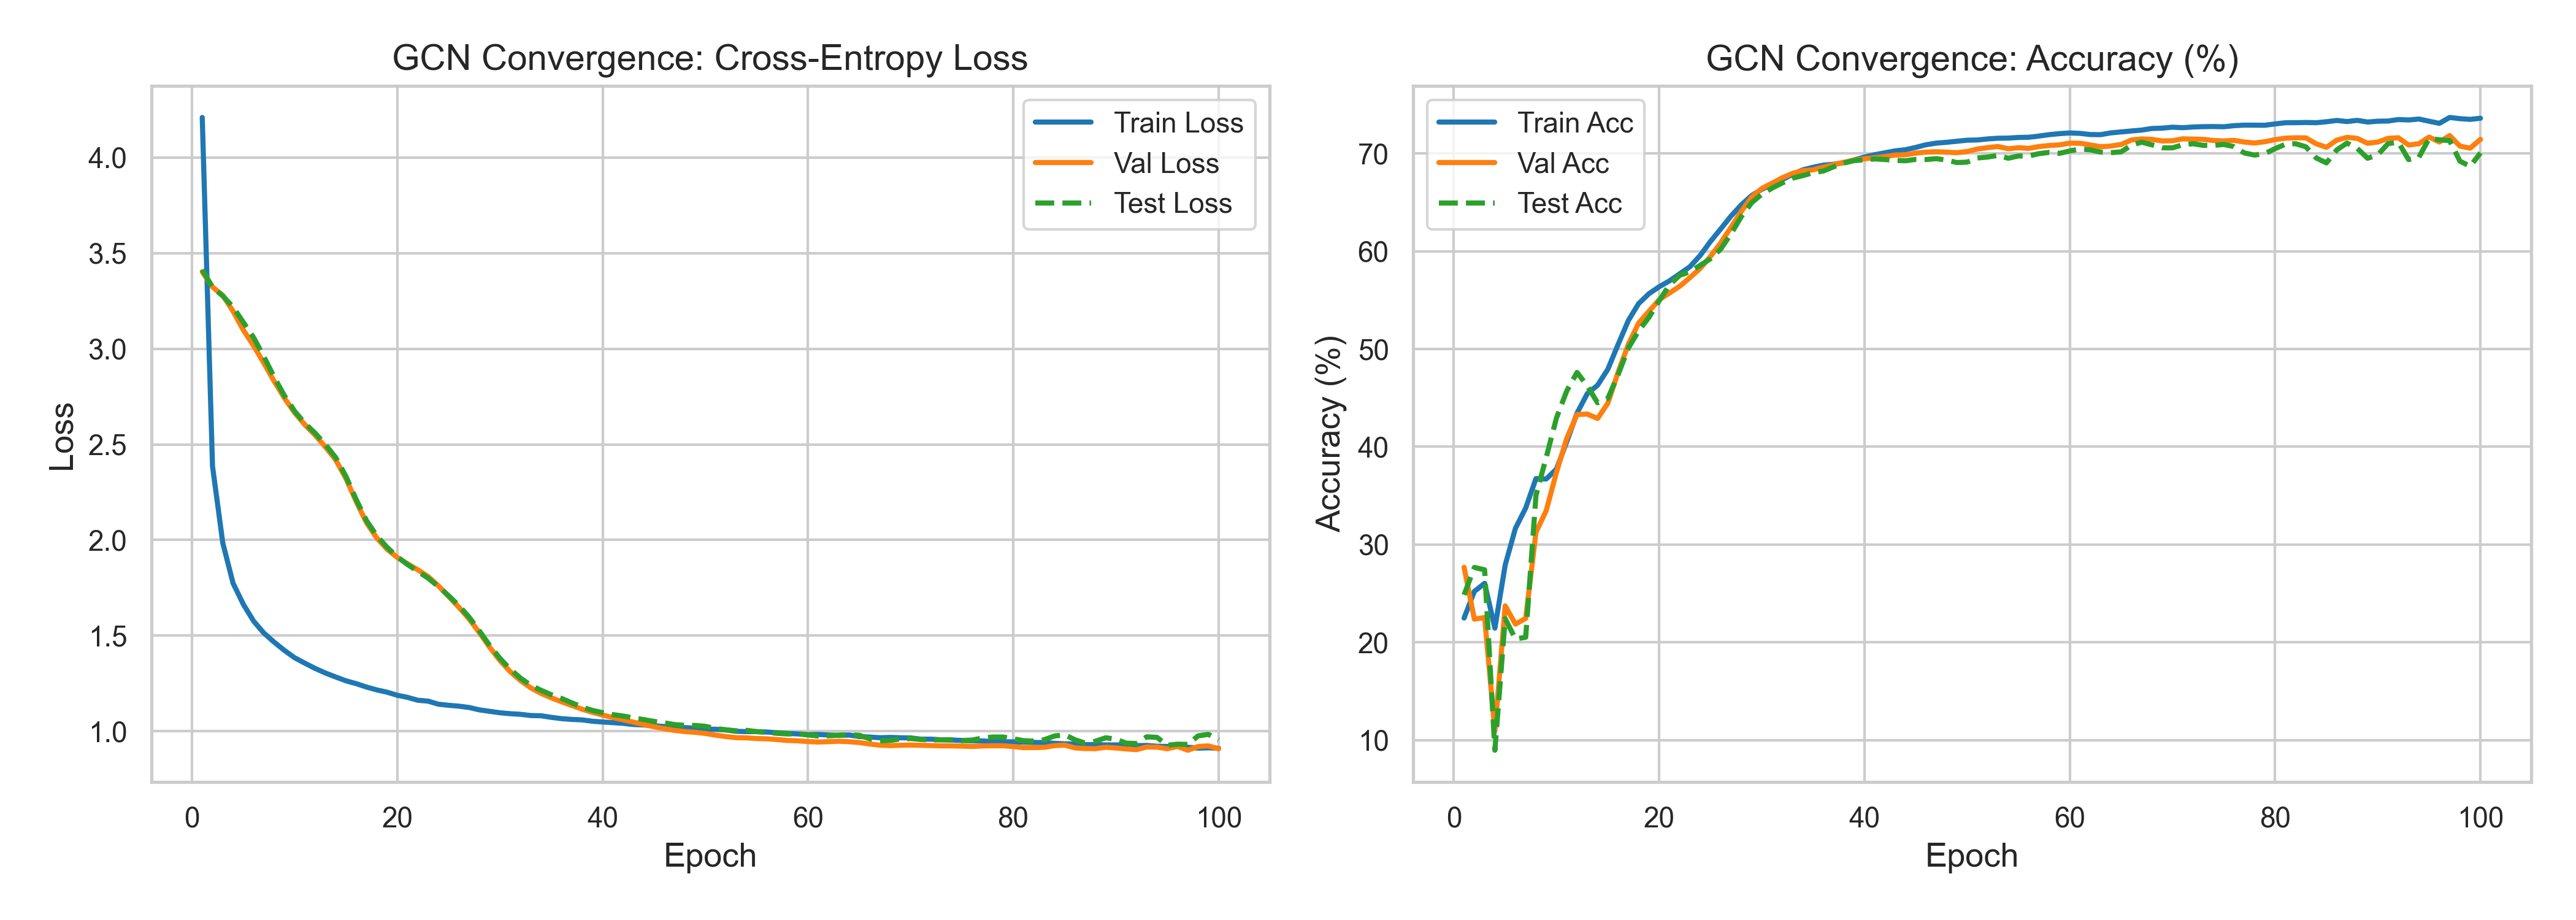
\includegraphics[width=0.98\columnwidth]{gcn_convergence.png}
    \caption{Training, validation, and test loss/accuracy for 3-layer GCN on
             \texttt{ogbn-arxiv} (100 epochs, lr=0.01, seed 42).}
    \label{fig:gcn_conv}
\end{figure}

\subsection{Convergence Dynamics}
Figure~\ref{fig:gcn_conv} shows GCN convergence over 100 epochs.  Training loss
falls rapidly from $4.21$ (epoch 1) to $\approx 0.91$ (epoch 100), while
validation loss exhibits high variance in the first 15 epochs before stabilizing.
The train--validation accuracy gap widens gradually after epoch 60 (training
accuracy with dropout inactive reaches $\approx 73.6\%$ while validation
plateaus), reflecting mild overfitting typical of citation-network GCNs without
label-propagation regularization.

The 100-epoch baseline achieves a peak validation accuracy of \textbf{71.82\%}
and a test accuracy of \textbf{71.30\%} at the best-validation epoch. To quantify run-to-run
variation, we repeated training under five random seeds (42--46); the
mean$\pm$std results are:
\begin{center}
  \small
  Test: $71.15\% \pm 0.26\%$ \quad Val: $71.92\% \pm 0.10\%$
\end{center}
This falls within ${\approx}0.6$ percentage points (pp) of the official OGB
GCN baseline ($71.74\% \pm 0.29\%$), confirming robust reproduction at 100
epochs vs.\ the reference 500-epoch run.

\subsection{Hyperparameter Sensitivity Analysis}

\begin{table}[htbp]
\centering
\caption{GCN Depth ($L$) and Learning Rate ($\eta$) ablation on
\texttt{ogbn-arxiv}. All ablations: 80 epochs, seed 42.
\textbf{Bold}: val-best within group. \textit{Italics}: 100-ep baseline.
Epoch times show $\approx{\pm}30\%$ GPU scheduling noise; depth trend is approximate.}
\label{tab:gcn_ablation}
\resizebox{\columnwidth}{!}{%
\begin{tabular}{lcccc}
\toprule
\textbf{Configuration} & \textbf{Val (\%)} & \textbf{Test (\%)} & \textbf{Mem (MB)} & \textbf{ms/ep} \\
\midrule
Depth $L = 2$               & 70.55 & 69.66 & 5{,}445.7 & 10.0 \\
Depth $L = 3$ (80 ep)       & 71.49 & 70.88 & 6{,}030.5 & 17.0 \\
\textit{$L=3$ (100 ep base)} & \textit{71.82} & \textit{71.30} & \textit{6{,}030.5} & \textit{14.5} \\
\textbf{Depth $L = 4$}       & \textbf{71.60} & 70.65 & 6{,}616.2 & 15.6 \\
Depth $L = 5$               & 71.04 & 70.08 & 7{,}201.7 & 18.9 \\
Depth $L = 6$               & 70.32 & 69.72 & 7{,}788.0 & 22.3 \\
\midrule
LR $\eta = 0.001$           & 68.91 & 67.71 & 6{,}030.5 & 14.6 \\
\textbf{LR $\eta = 0.005$}  & \textbf{71.63} & 70.87 & 6{,}030.5 & 13.5 \\
LR $\eta = 0.010$ (80 ep)   & 71.49 & 70.88 & 6{,}030.5 & 17.0 \\
LR $\eta = 0.050$           & 69.33 & 68.17 & 6{,}030.5 & 13.2 \\
\bottomrule
\end{tabular}%
}
\end{table}

\begin{figure}[htbp]
    \centering
    \begin{subfigure}[b]{0.48\columnwidth}
        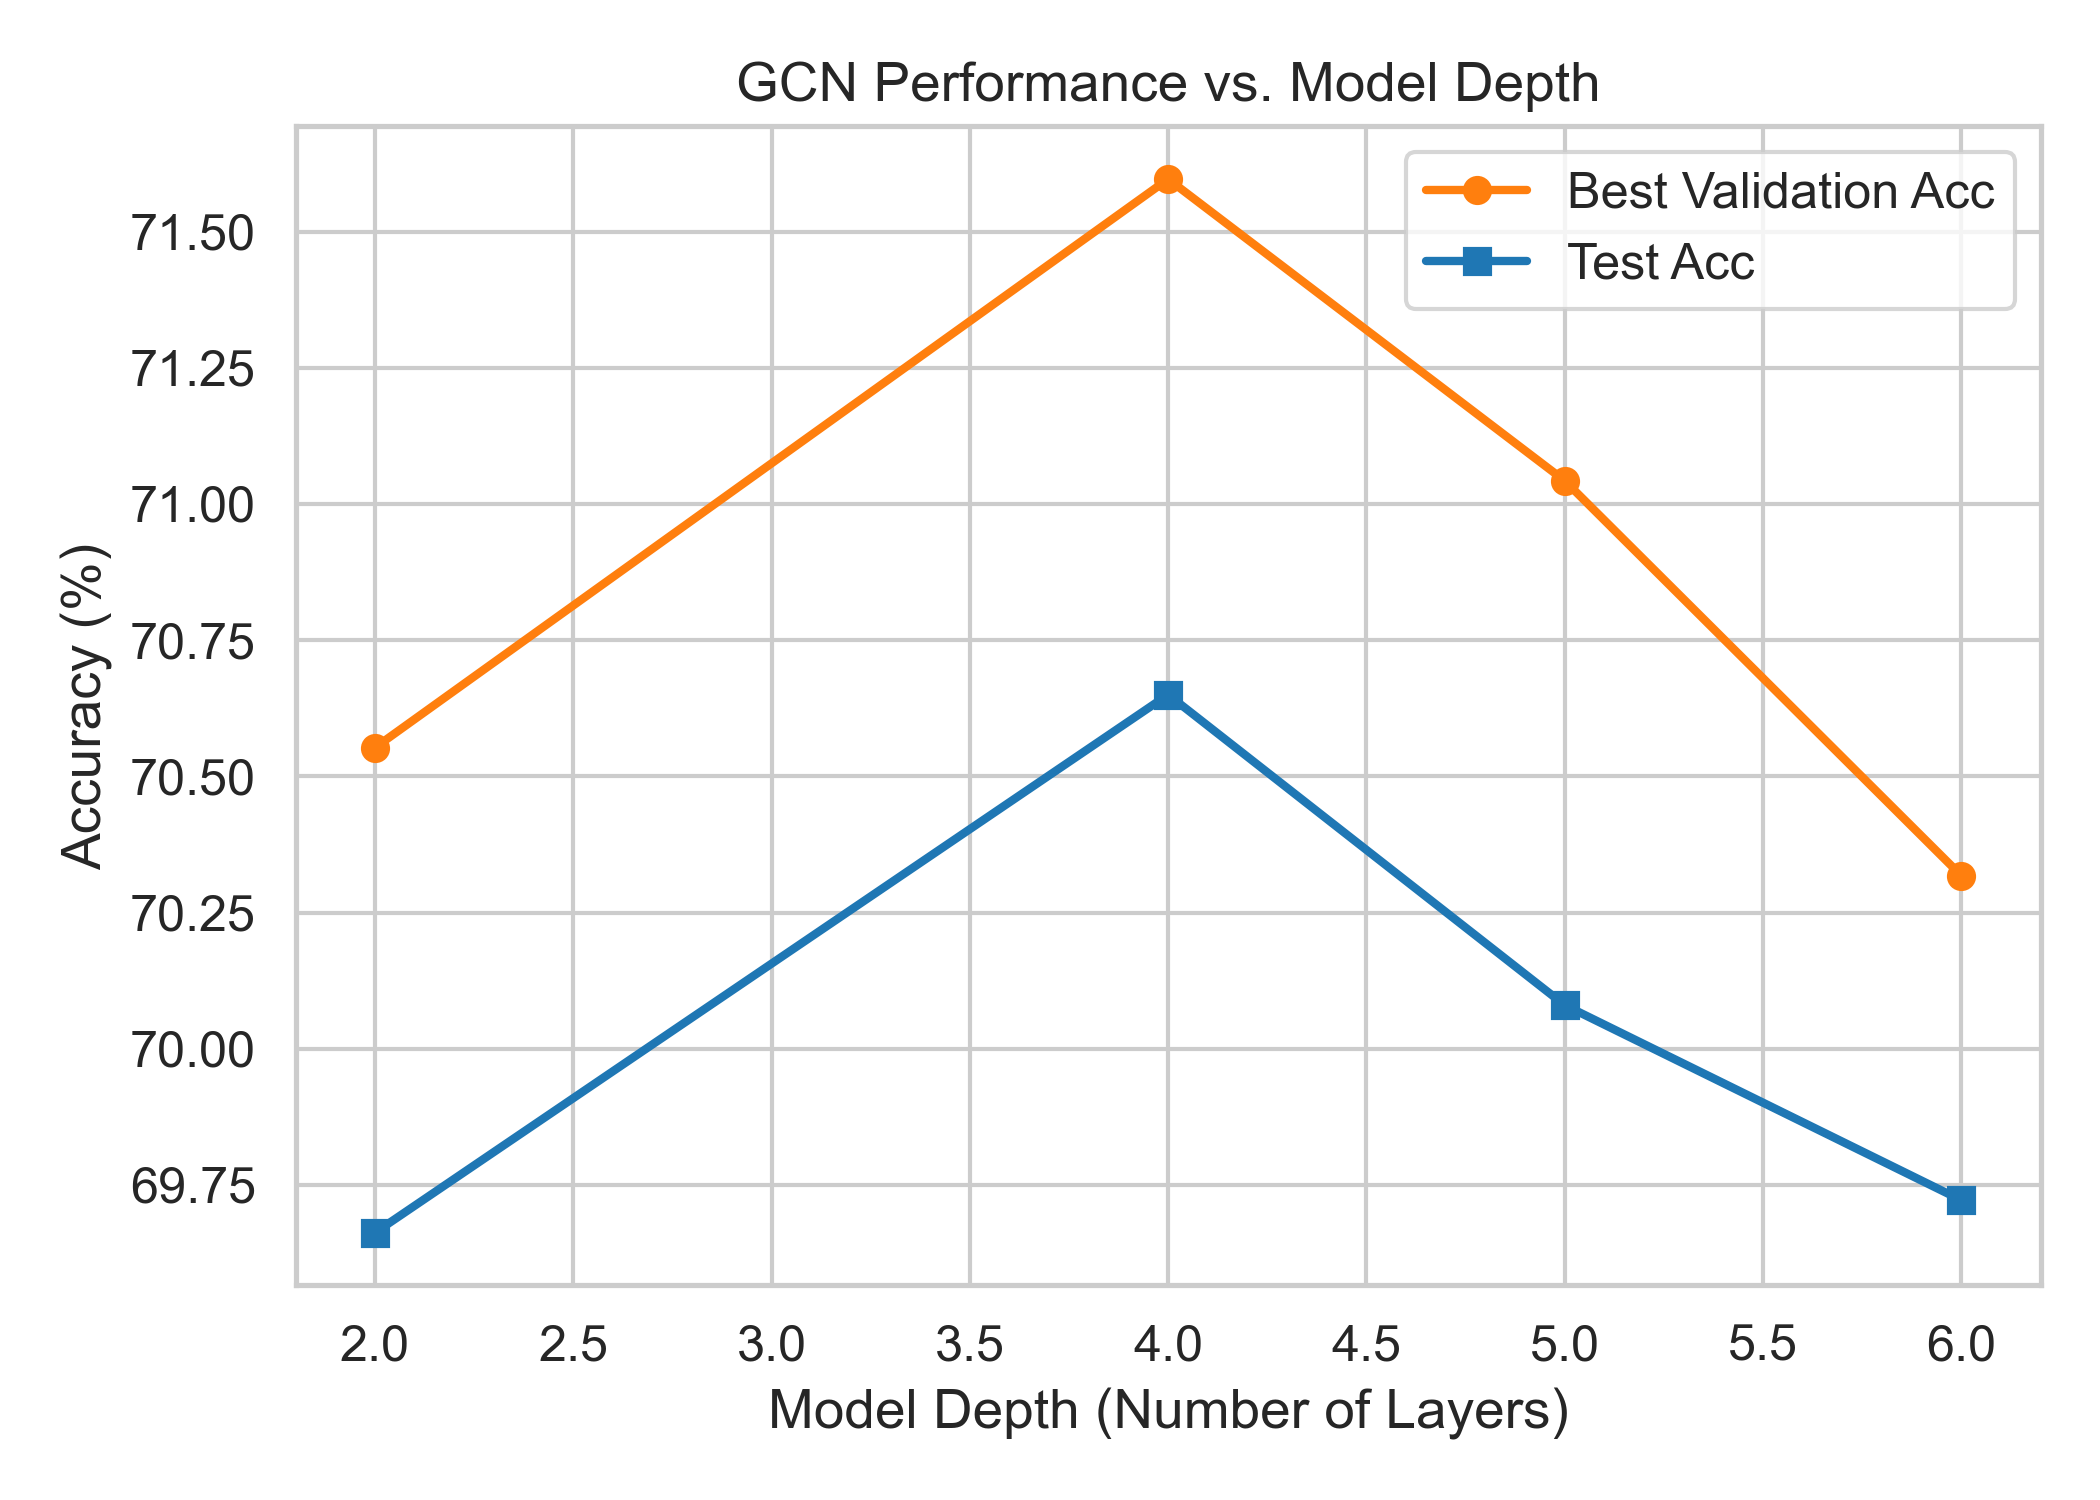
\includegraphics[width=\linewidth]{gcn_depth_ablation.png}
        \caption{Depth ($L$)}
    \end{subfigure}
    \hfill
    \begin{subfigure}[b]{0.48\columnwidth}
        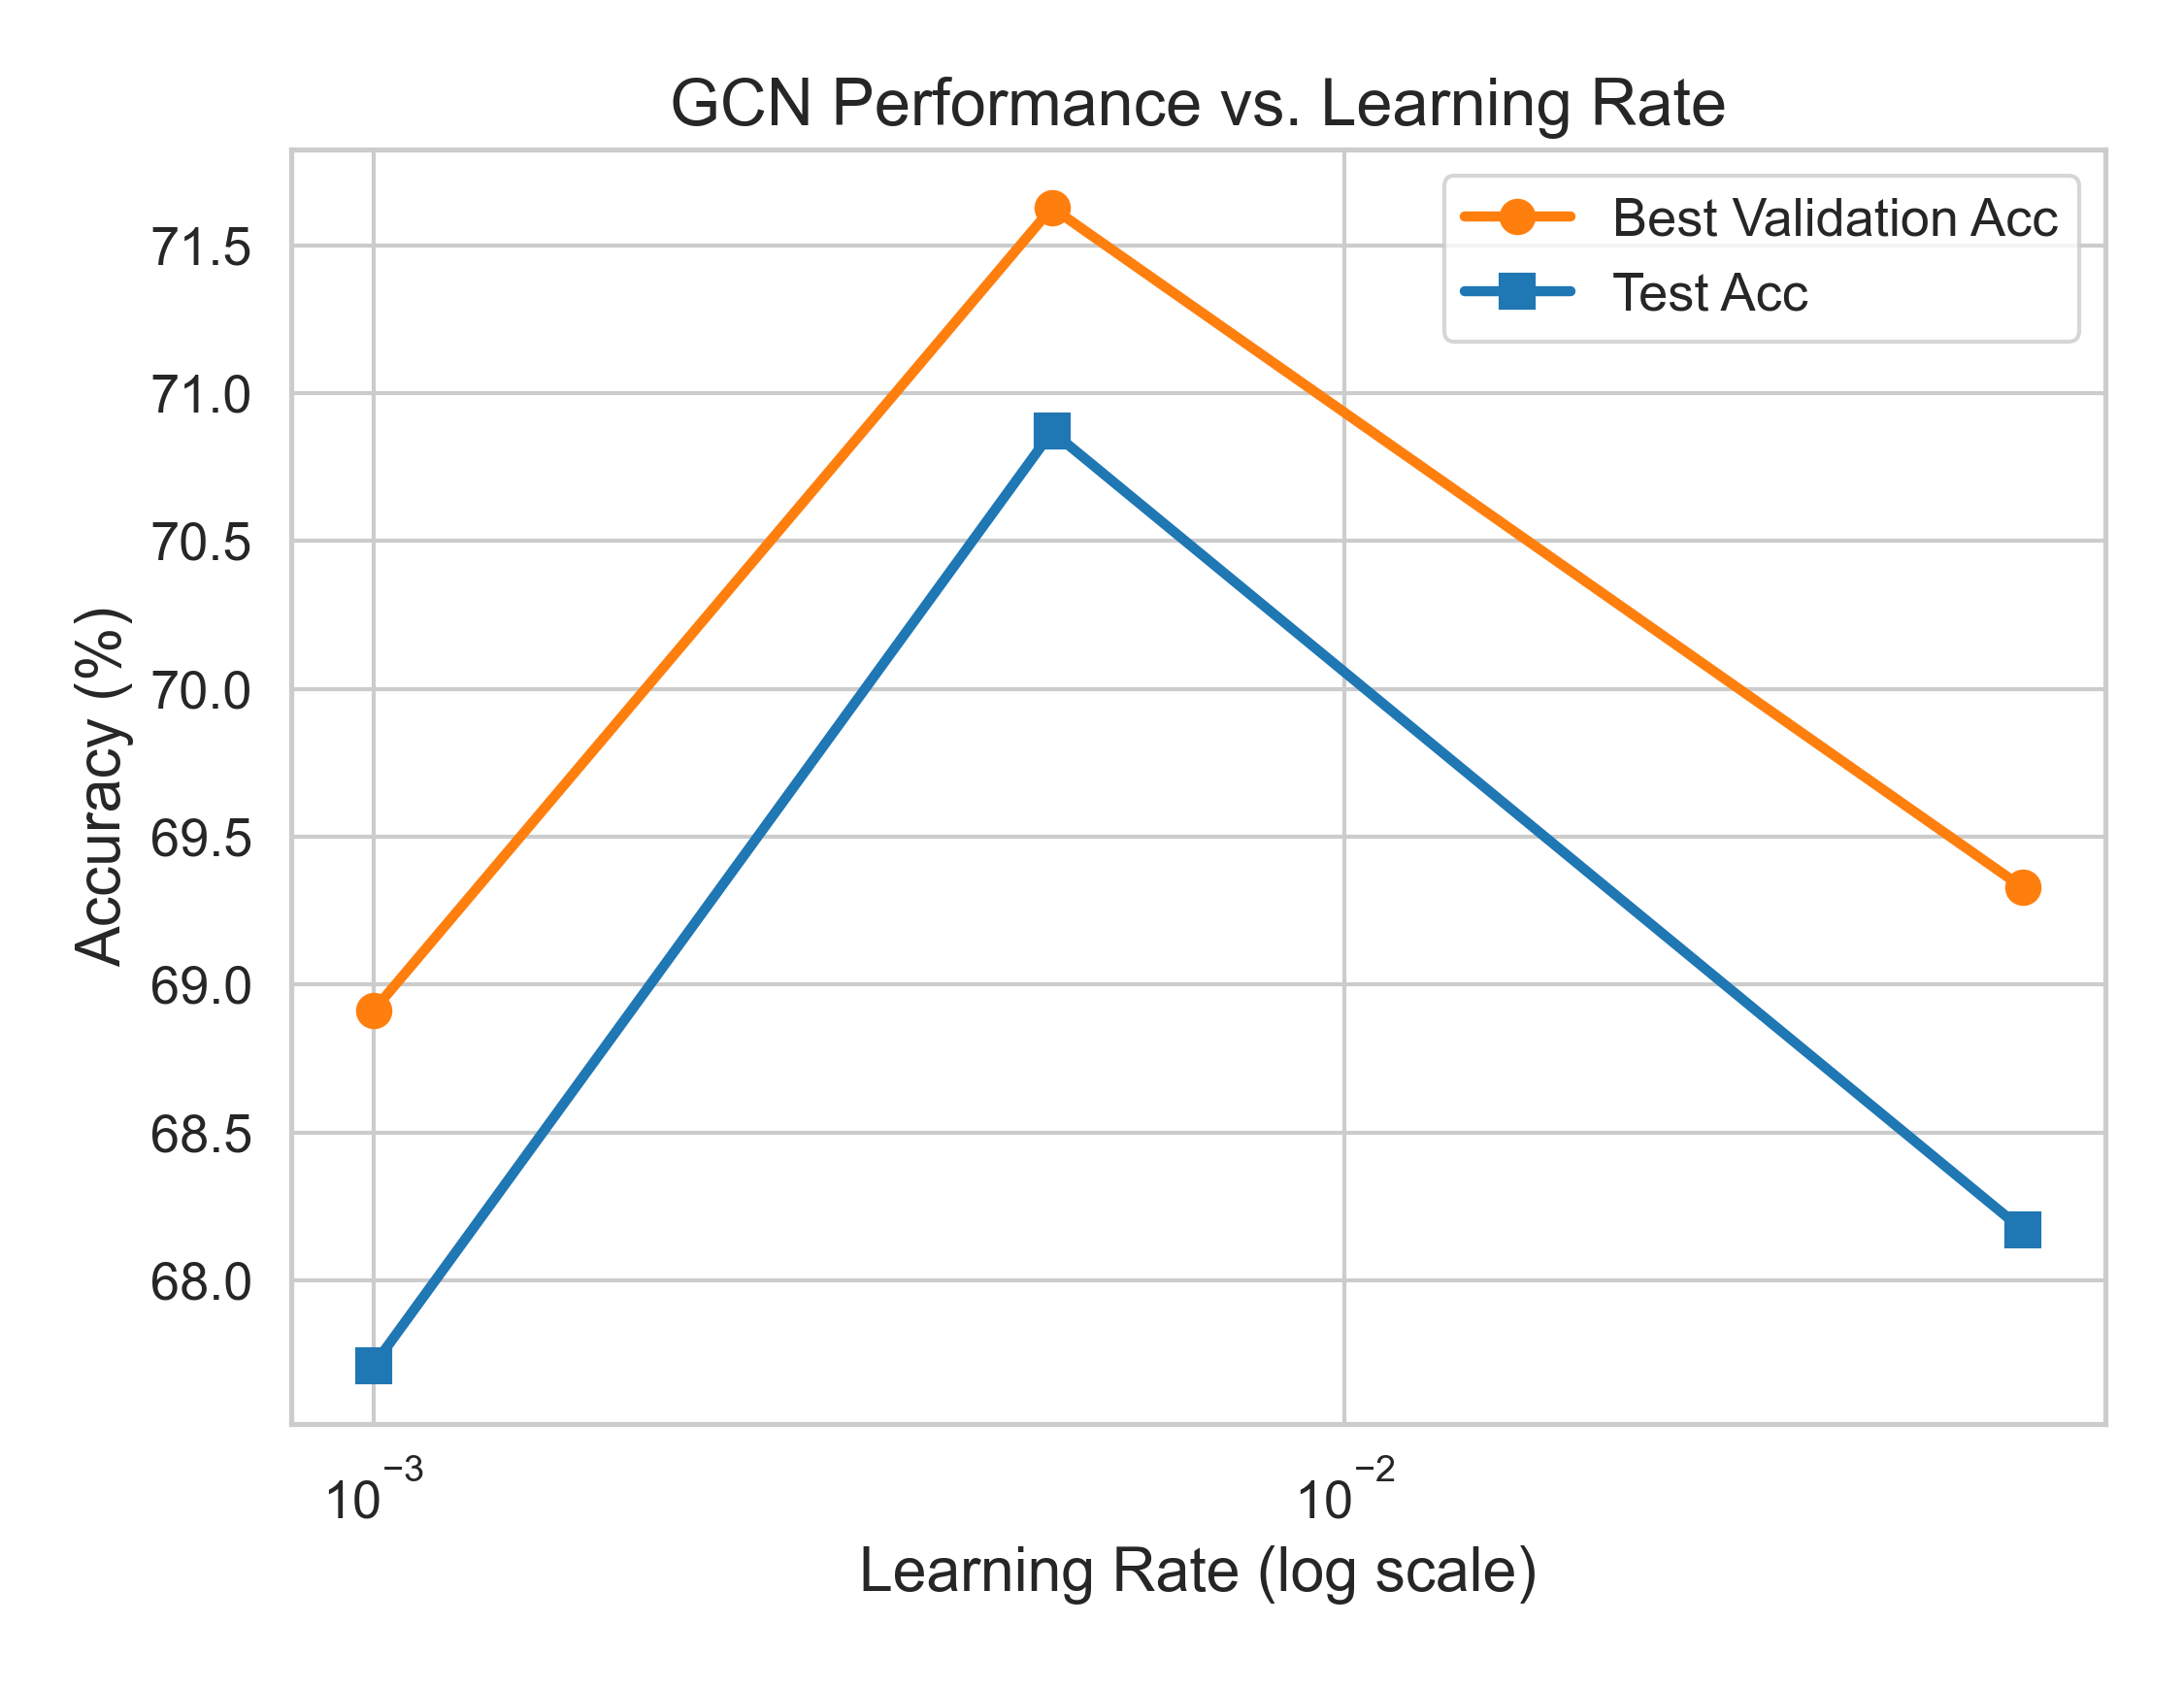
\includegraphics[width=\linewidth]{gcn_lr_ablation.png}
        \caption{LR ($\eta$)}
    \end{subfigure}
    \caption{GCN validation and test accuracy at 80 epochs across (a) model depths and
             (b) learning rates on \texttt{ogbn-arxiv}.}
    \label{fig:gcn_ablations}
\end{figure}

\paragraph{Impact of Model Depth ($L$):}
Increasing depth from $L=2$ to $L=3$ expands the receptive field by one hop,
improving test accuracy by $1.22$ pp ($69.66\%{\to}70.88\%$) -- a gain
${\approx}4.7{\times}$ the measured test standard deviation ($\sigma_{\text{test}}
\approx 0.26$ pp from 100-epoch 3-layer runs), suggesting a real effect.
At $L=4$, validation accuracy peaks ($71.60\%$), but the $0.11$ pp margin over $L=3$ ($71.49\%$) is comparable
to the observed validation noise ($\sigma_{\text{val}} \approx 0.10$ pp), so the
improvement is not significant.  Beyond $L=4$, performance drops monotonically:
val accuracy falls from $71.60\%$ at $L=4$ to $70.32\%$ at $L=6$ (a $1.28$ pp
drop, ${\approx}13{\times}\sigma_{\text{val}}$), indicating genuine degradation.

We hypothesize this degradation stems from a combination of \emph{oversmoothing}
and optimization difficulty.  The GCN propagation rule
\begin{equation}
  H^{(l+1)} = \sigma\!\left(\tilde{D}^{-\frac{1}{2}}\tilde{A}\tilde{D}^{-\frac{1}{2}}
               H^{(l)} W^{(l)}\right)
  \label{eq:gcn_layer}
\end{equation}
repeatedly averages node representations over expanding neighborhoods, which may
drive them toward stationary eigenvectors and erode class-discriminative structure.
Batch normalization mitigates intra-layer covariate shift but may not fully
counteract Dirichlet energy decay; gradient attenuation across deep stacks is an
equally plausible contributor, and distinguishing the two would require explicit
feature-variance or Dirichlet-energy measurements.

Peak GPU memory (measured via \texttt{torch.cuda.max\_memory\_allocated})
grows linearly by ${\approx}585$ MiB per additional layer (from $5{,}446$ MiB at
$L=2$ to $7{,}788$ MiB at $L=6$) as PyTorch caches intermediate activation
tensors for backpropagation.

\paragraph{Impact of Learning Rate ($\eta$):}
At $\eta=0.001$, training is too slow to converge in 80 epochs ($68.91\%$ val).
At $\eta=0.05$, excessive gradient steps cause oscillation and premature
saturation ($69.33\%$ val).  The plateau between $\eta=0.005$ and $\eta=0.010$
is nearly flat ($71.63\%$ vs.\ $71.49\%$ val; test gap $=0.01$ pp), well below
the empirical noise floor ($\sigma_{\text{test}}\approx 0.26$ pp), suggesting
that learning rate has limited marginal effect in this range.  Epoch runtimes
vary by only $\approx 4$ ms across all LR settings, reflecting GPU scheduling
noise rather than algorithmic differences.

% =============================================================================
\section{Task 2: Mini-Batch GraphSAGE \& Neighborhood Sampling}
% =============================================================================

\subsection{Experimental Configuration}
GraphSAGE was evaluated on the large-scale \texttt{ogbn-products} co-purchasing
graph ($|V|=2{,}449{,}029$, $|E|=61{,}859{,}140$, 47 product categories). The
architecture uses 3 GraphSAGE layers ($d=256$, mean aggregation, dropout $p=0.5$,
batch normalization), trained with Adam ($\eta=0.003$). The baseline uses
batch size $B=1{,}024$ and per-layer fanouts $S=[15,10,5]$ for 15 epochs. To
prevent neighborhood explosion in evaluation, inference also uses the same
sampler with eval batch size $B_{\text{eval}}=4{,}096$.

\begin{figure}[htbp]
    \centering
    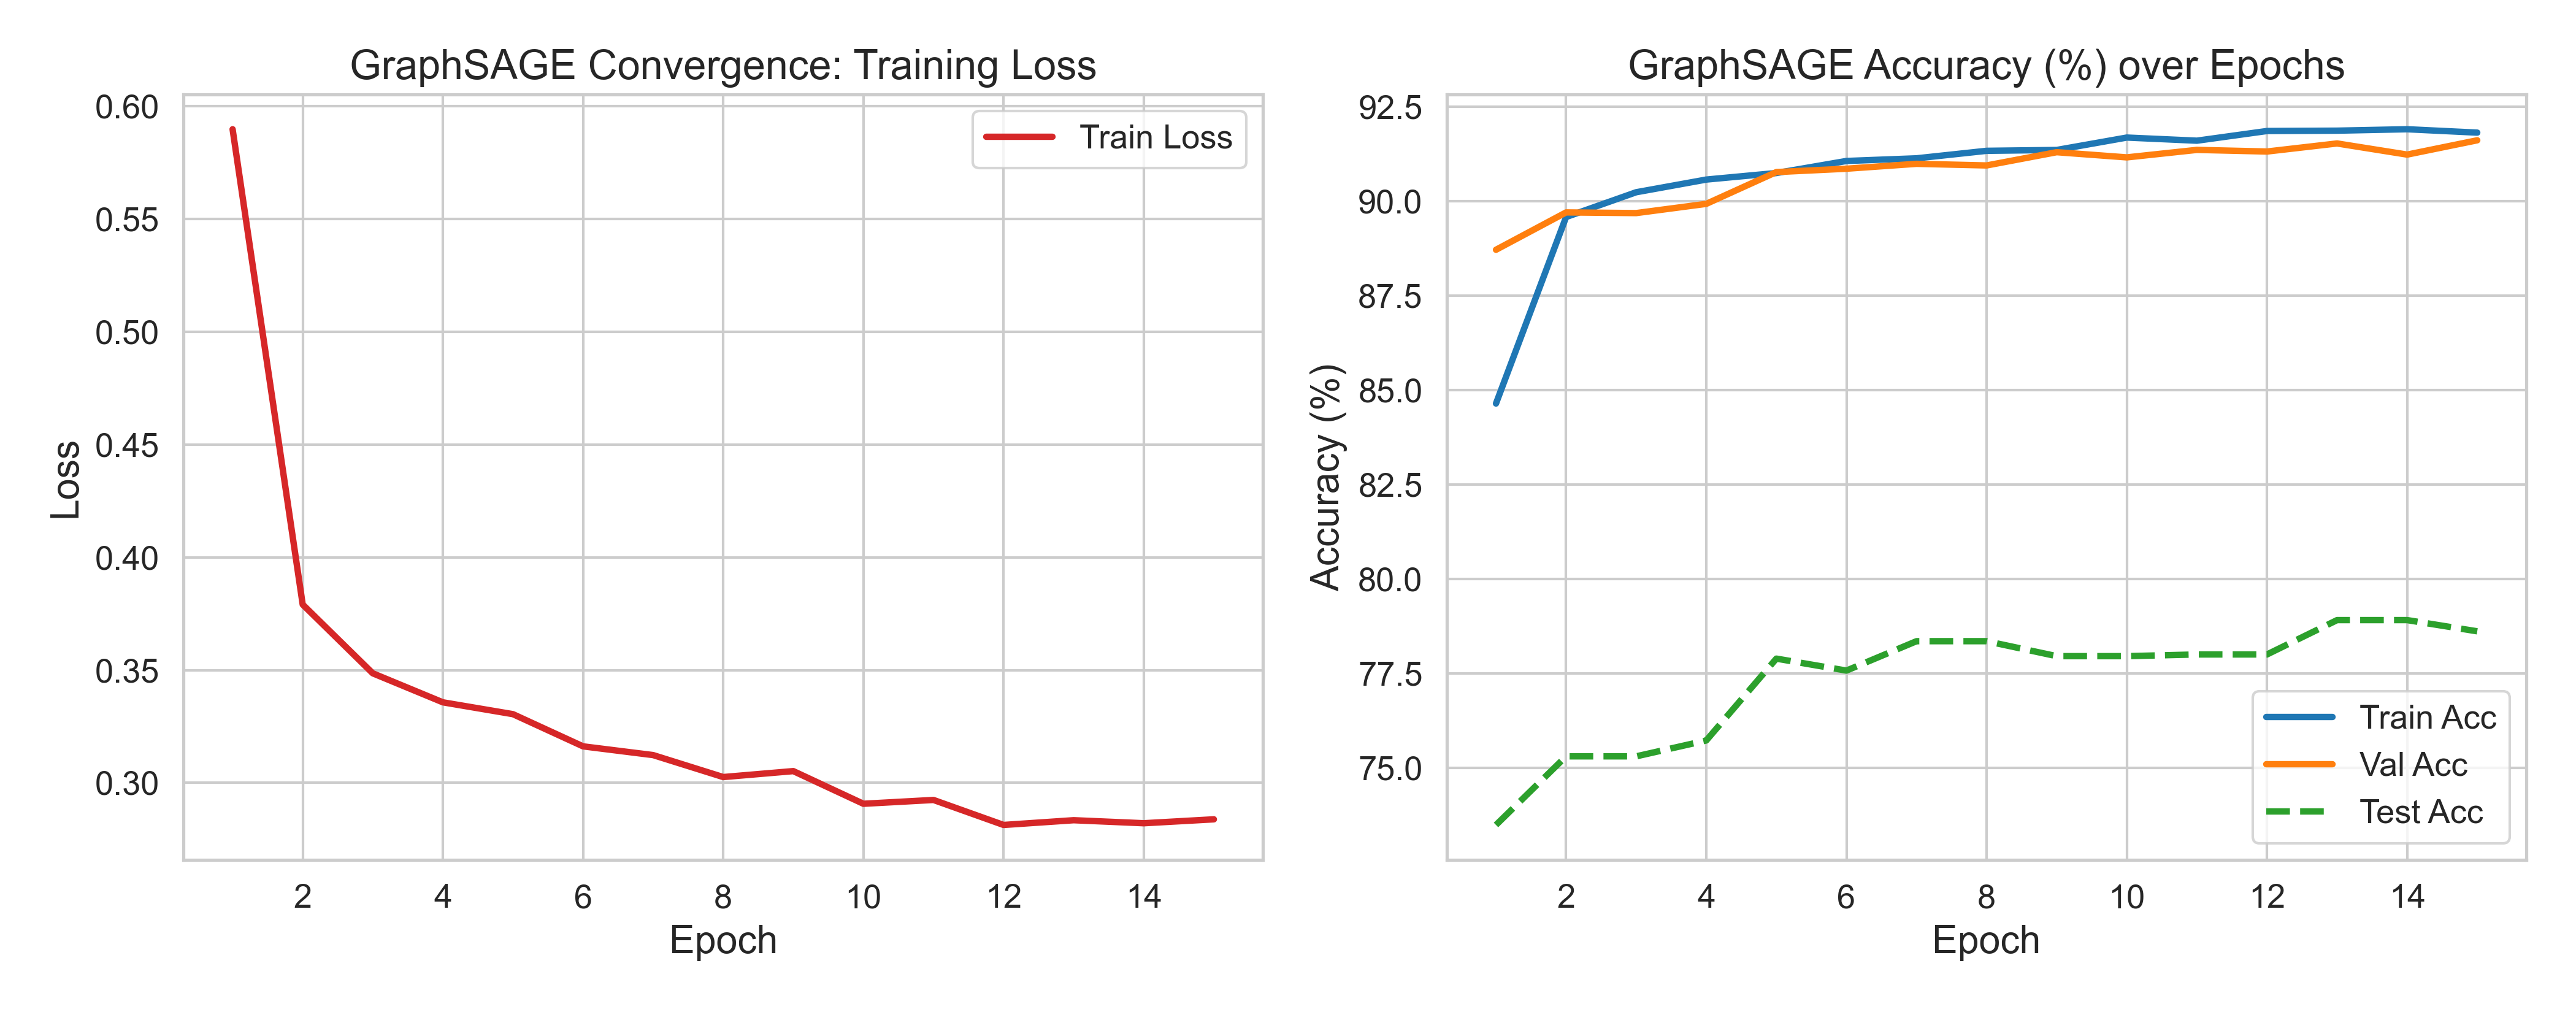
\includegraphics[width=0.98\columnwidth]{sage_convergence.png}
    \caption{GraphSAGE train/val/test accuracy and training loss on
             \texttt{ogbn-products} ($B=1{,}024$, $S=[15,10,5]$, 15 epochs).}
    \label{fig:sage_conv}
\end{figure}

\subsection{Convergence \& Replication}
GraphSAGE converged steadily over 15 epochs (Figure~\ref{fig:sage_conv}),
reaching a best validation accuracy of \textbf{91.61\%} and a test accuracy of
\textbf{78.61\%} at the best-validation epoch -- within $0.09$ pp of the
official OGB GraphSAGE baseline ($78.70\% \pm 0.36\%$), confirming a
near-exact reproduction.

The large validation--test gap ($91.61\%$ vs.\ $78.61\%$) is \emph{expected}:
OGB products uses a sales-ranking-based split in which popular (high-sales-rank)
products dominate the training set and niche (tail) products form the test set,
creating an intentional distribution shift that makes validation performance a
poor proxy for test performance. Additionally, our evaluation uses the same
neighbor sampler as training rather than OGB's full-neighbor inference; this
deviates from the official protocol but was chosen for speed and memory, and
may introduce a small accuracy gap relative to the reported $78.70\%$ baseline.

\subsection{Sampling Hyperparameter Investigation}
All ablation runs used an identical 5-epoch budget. For \emph{fanout} ablations
(fixed $B{=}1{,}024$), all configurations see the same number of gradient steps
($\approx193$/epoch). For \emph{batch-size} ablations, step counts differ by
design ($B{=}512$: $\approx385$ steps/ep; $B{=}2{,}048$: $\approx97$ steps/ep);
we compare convergence within the same epoch budget, not the same update count
(Table~\ref{tab:sage_ablation}). We expect that accuracy on extended runs would further
favor configurations with adequate neighbor coverage.

\begin{table}[htbp]
\centering
\caption{GraphSAGE Batch Size ($B$) and Fanout ($S$) ablation on
\texttt{ogbn-products}. All ablations: 5 epochs, seed 42.
\textbf{Bold}: best within 5-ep ablations. \textit{Italics}: 15-ep baseline.}
\label{tab:sage_ablation}
\resizebox{\columnwidth}{!}{%
\begin{tabular}{lcccc}
\toprule
\textbf{Configuration} & \textbf{Val (\%)} & \textbf{Test (\%)} & \textbf{Mem (MB)} & \textbf{s/ep} \\
\midrule
Batch $B = 512$                          & \textbf{90.80} & 76.45 & 7{,}113.8 & 66.3 \\
Batch $B = 1{,}024$ (5 ep)              & 90.77 & \textbf{77.89} & \textbf{7{,}109.7} & 59.5 \\
\textit{$B=1{,}024$ (15 ep base)}        & \textit{91.61} & \textit{78.61} & \textit{7{,}109.7} & \textit{60.6} \\
Batch $B = 2{,}048$                      & 90.62 & 77.33 & 9{,}393.7 & \textbf{49.9} \\
\midrule
Fanout $S=[5, 5, 5]$                     & 89.05 & 75.92 & \textbf{3{,}735.0} & \textbf{16.9} \\
Fanout $S=[5, 5, 15]$                    & 89.27 & 75.52 & 5{,}539.7 & 35.4 \\
Fanout $S=[15, 5, 5]$                    & \textbf{90.80} & 77.29 & 5{,}454.2 & 37.3 \\
Fanout $S=[10, 10, 5]$                   & 90.37 & 77.24 & 6{,}152.9 & 46.8 \\
Fanout $S=[15, 10, 5]$ (5 ep)           & 90.77 & \textbf{77.89} & 7{,}109.7 & 59.5 \\
\bottomrule
\end{tabular}%
}
\end{table}

\begin{figure}[htbp]
    \centering
    \begin{subfigure}[b]{0.48\columnwidth}
        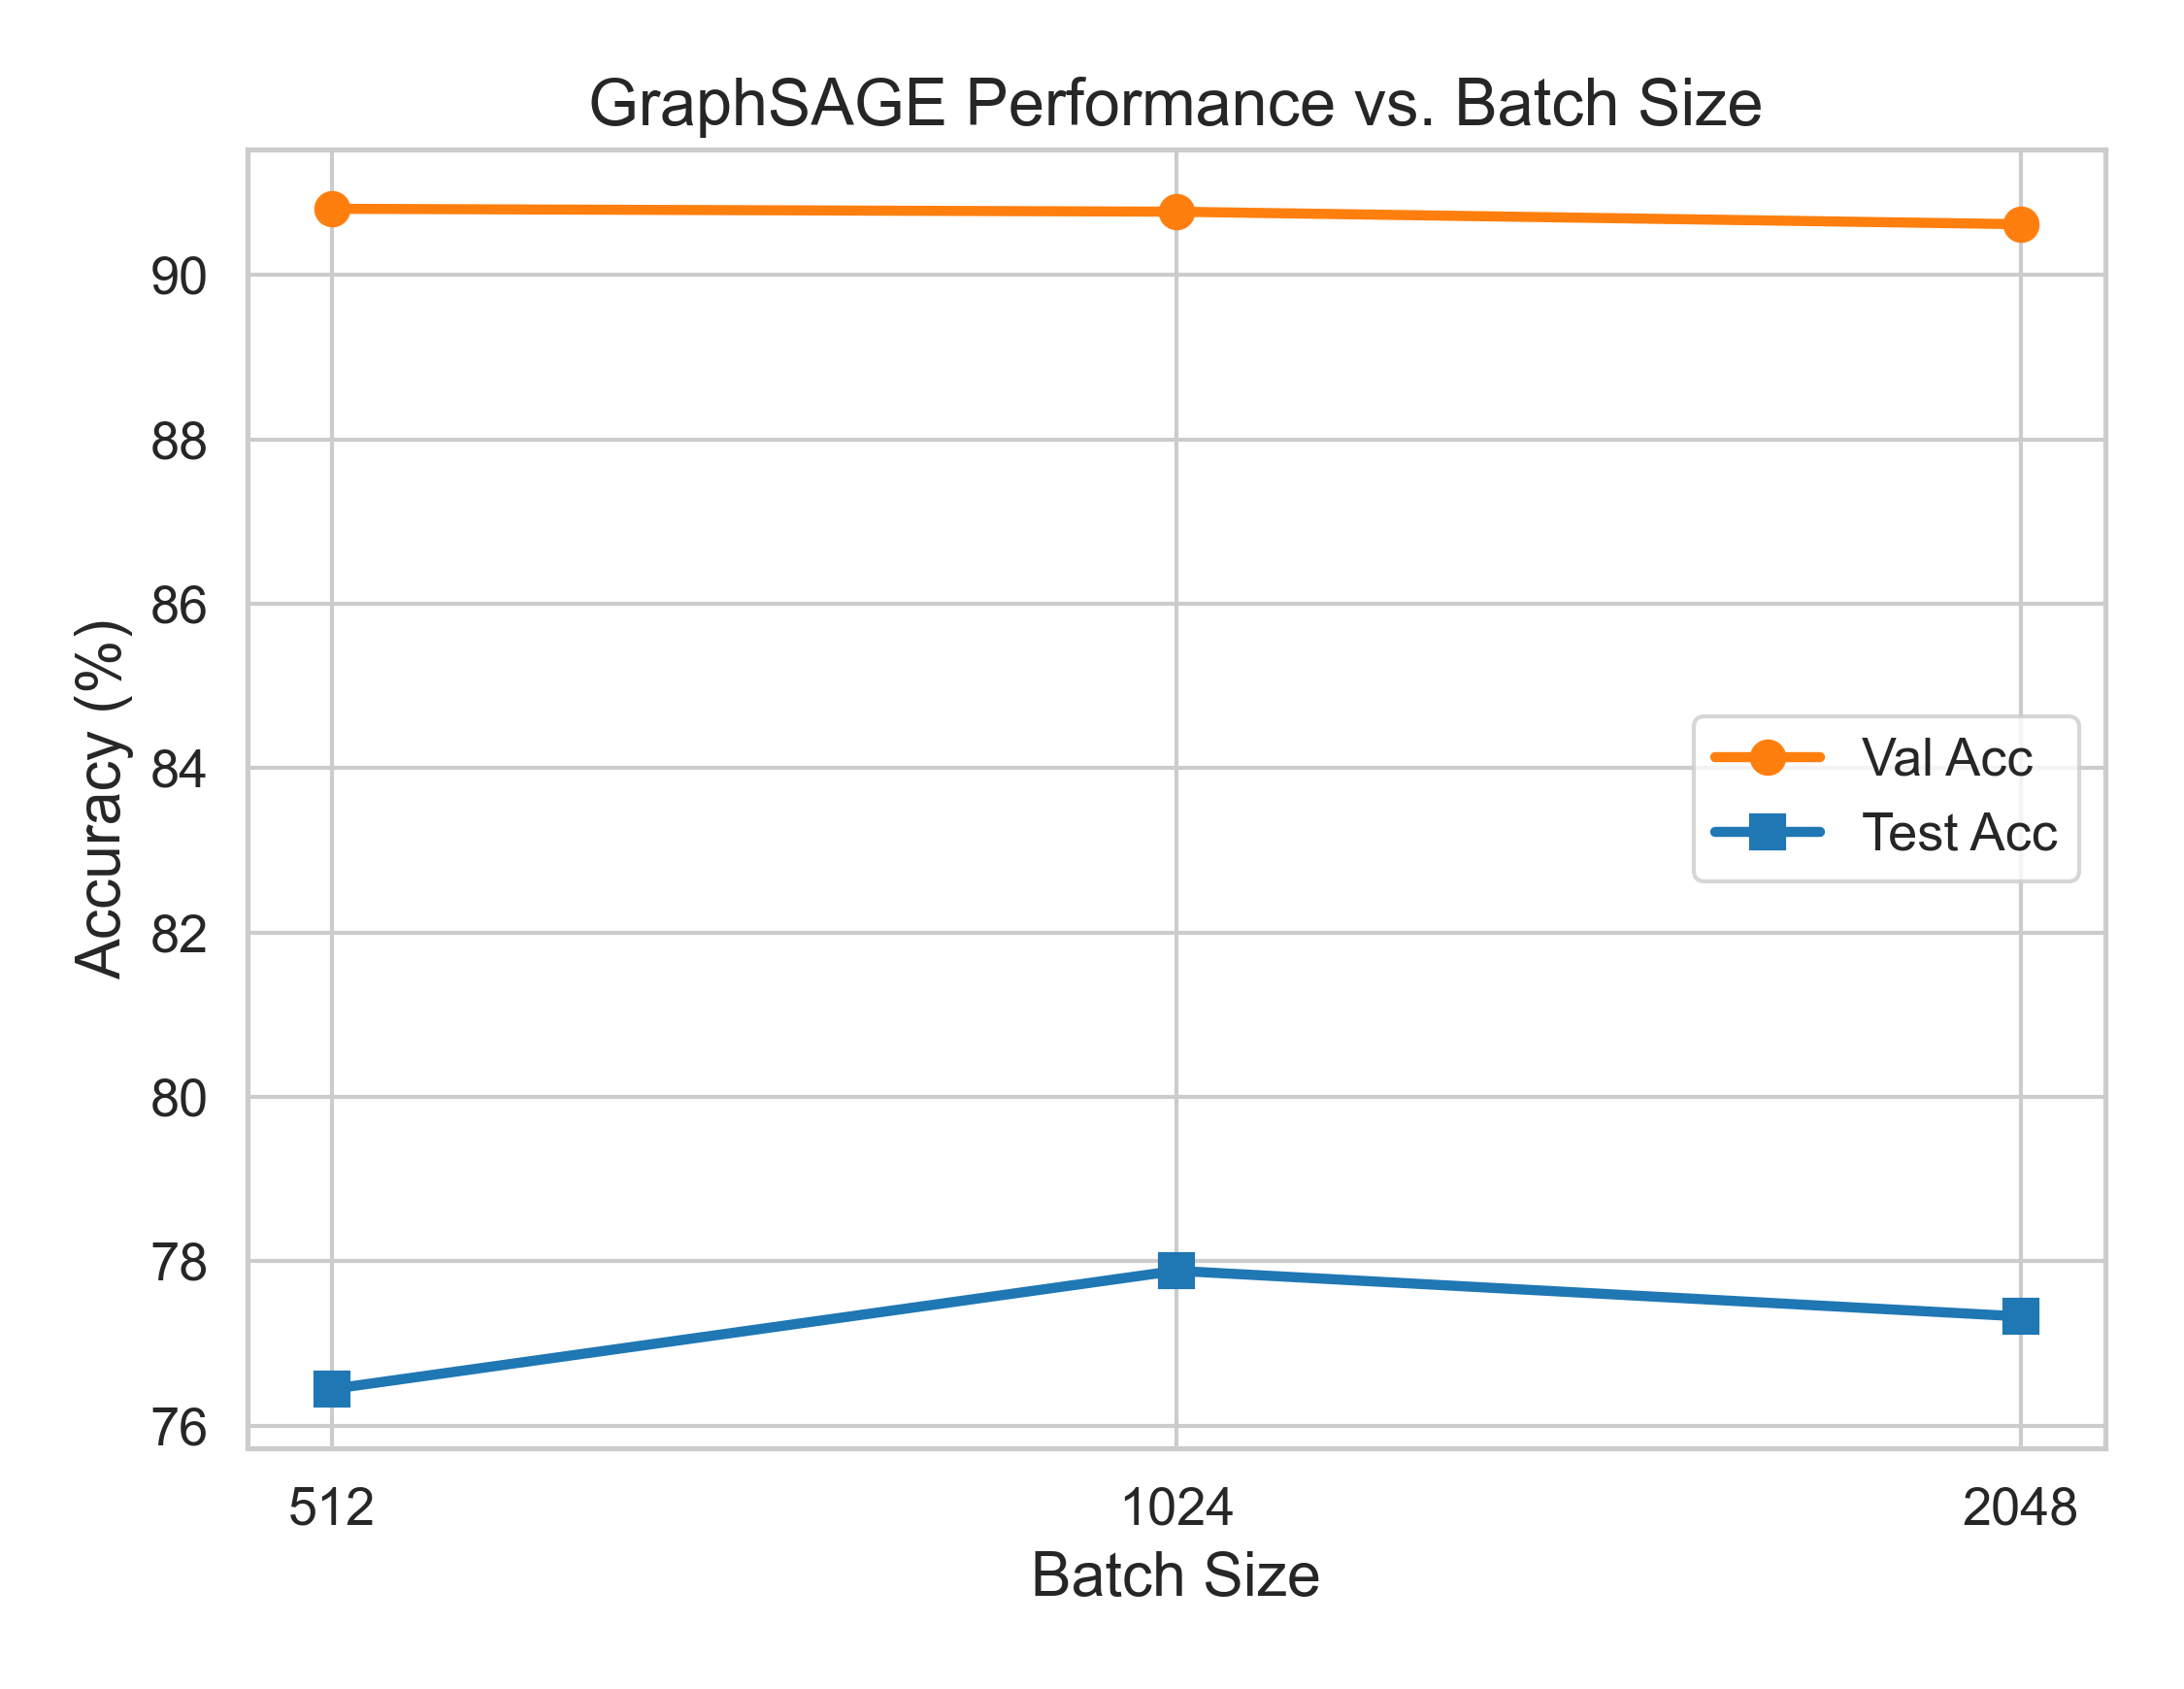
\includegraphics[width=\linewidth]{sage_batch_ablation.png}
        \caption{Batch Size ($B$)}
    \end{subfigure}
    \hfill
    \begin{subfigure}[b]{0.48\columnwidth}
        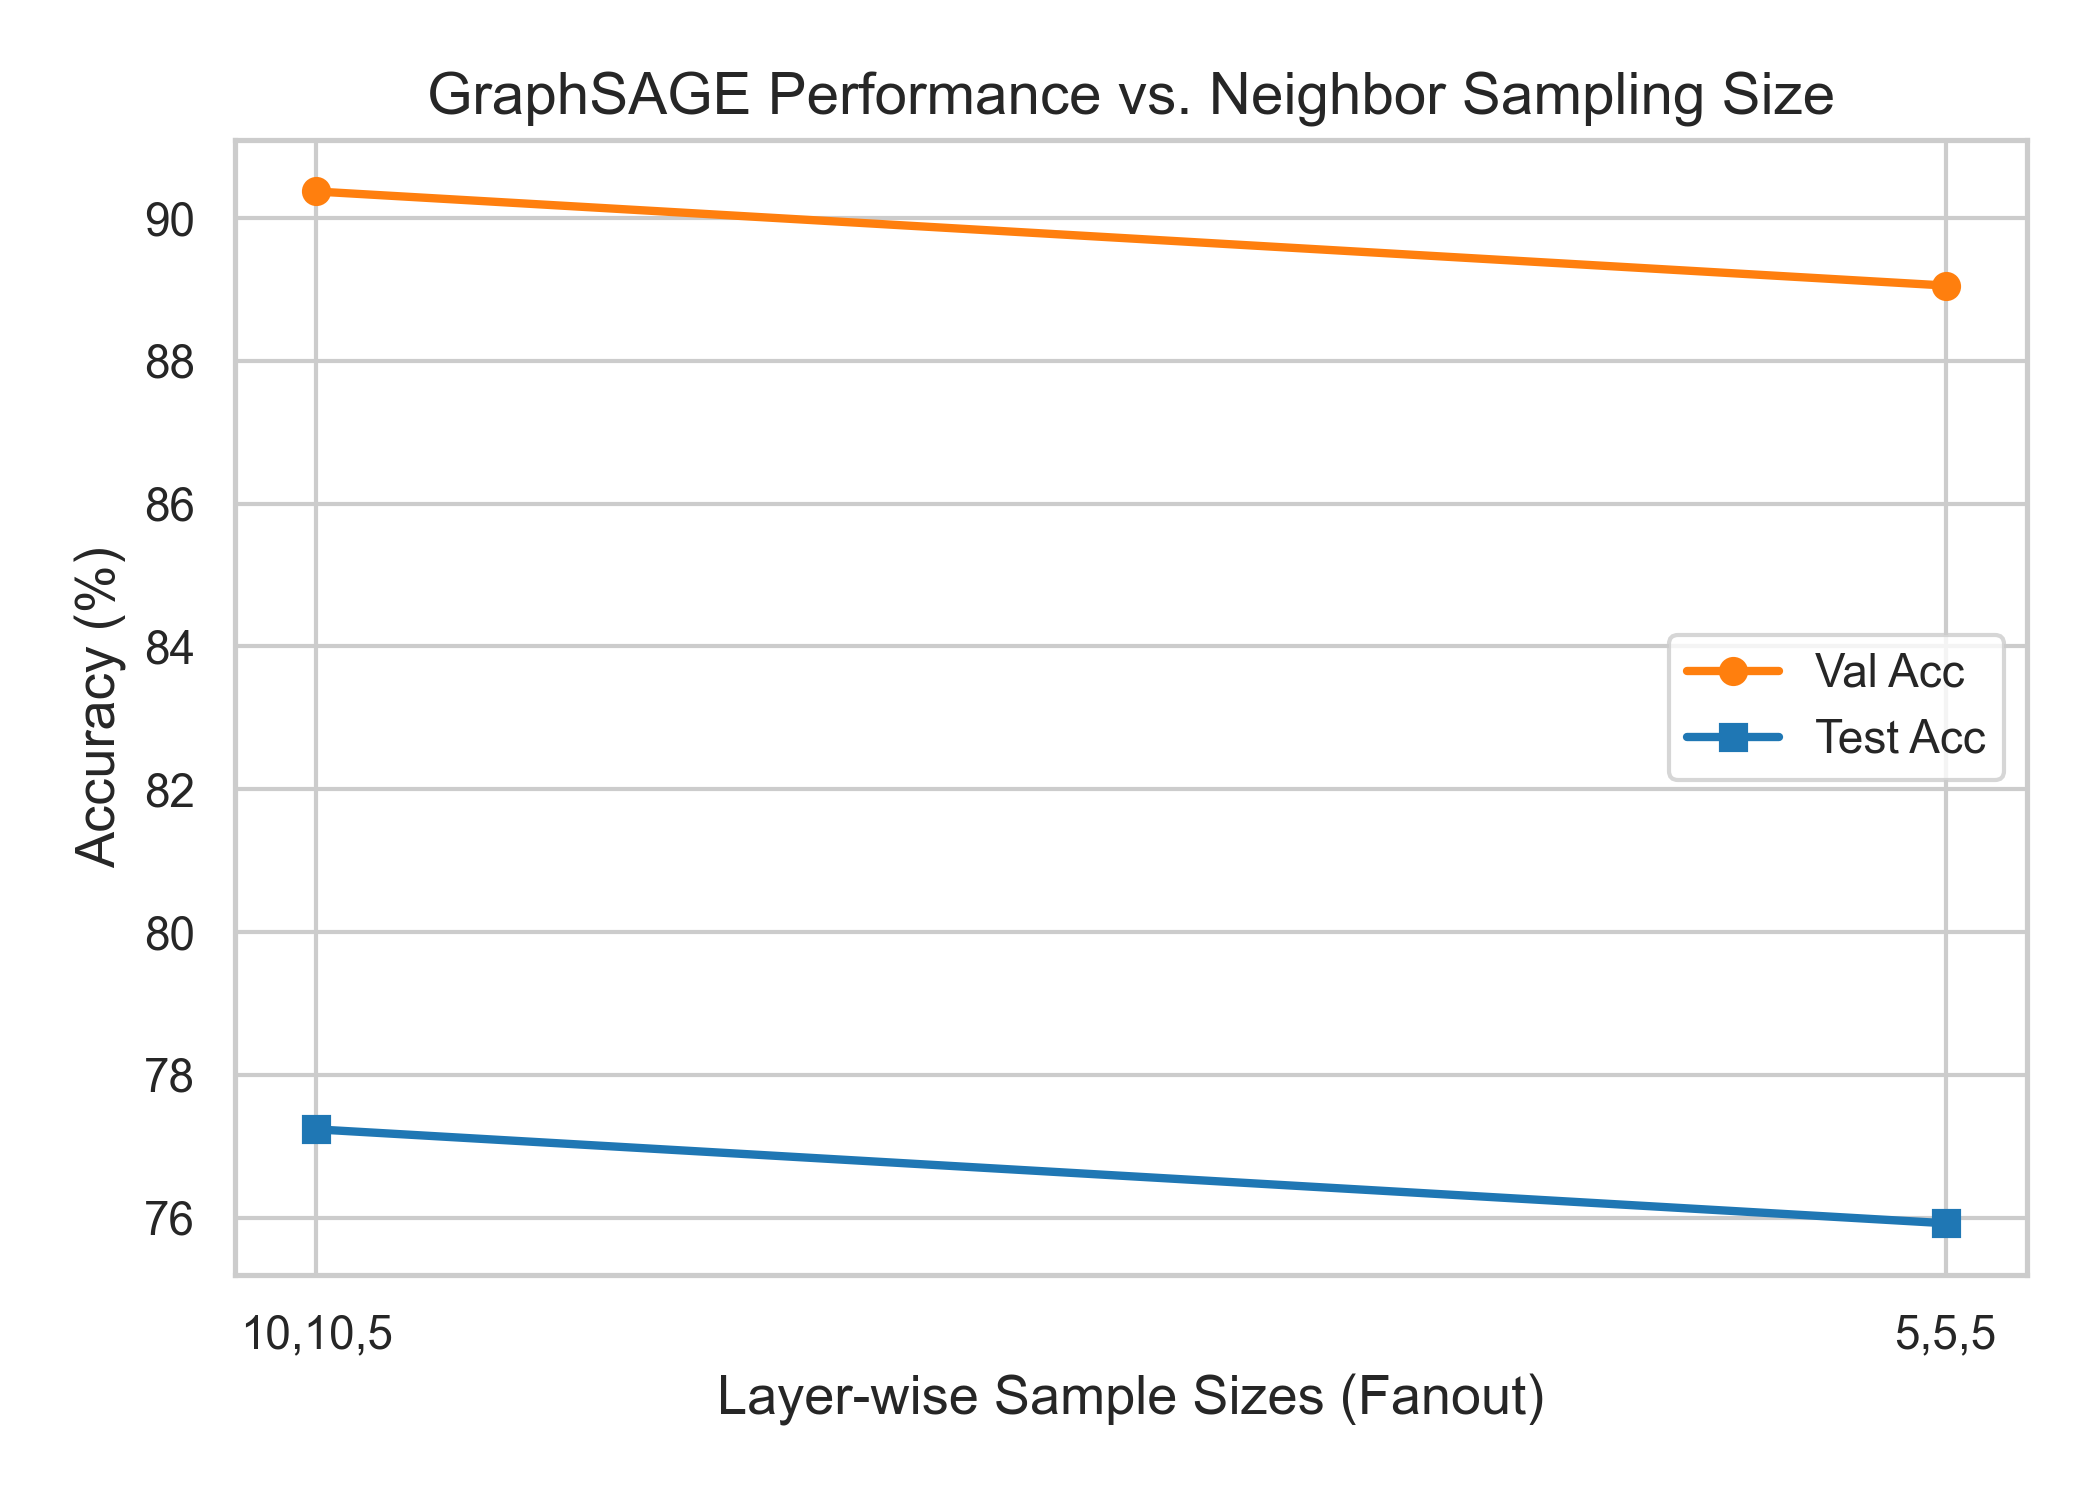
\includegraphics[width=\linewidth]{sage_sampling_ablation.png}
        \caption{Fanout ($S$)}
    \end{subfigure}
    \caption{GraphSAGE sensitivity to (a) mini-batch size and (b) neighbor
             fanout on \texttt{ogbn-products} (5-epoch budget).}
    \label{fig:sage_ablations}
\end{figure}

\paragraph{Impact of Batch Size ($B$):}
With $196{,}615$ training nodes, the number of gradient steps per epoch is
${\approx}385$ ($B{=}512$), $193$ ($B{=}1{,}024$), and $97$ ($B{=}2{,}048$).
Larger batches amortize per-step overhead (kernel launch, loop cost), reducing
epoch time from $66.3$s to $49.9$s ($1.3{\times}$ speedup). Peak memory is
tracked across the full epoch (training + evaluation) without a per-phase reset;
at $B{=}512$ and $B{=}1{,}024$ the evaluation pass ($B_{\text{eval}}{=}4{,}096$)
likely dominates the peak, keeping memory flat at ${\approx}7{,}110$ MB for
both. At $B{=}2{,}048$, the training frontier exceeds the evaluation footprint,
raising peak memory by $32\%$ to $9{,}394$ MB. Validation accuracy at 5 epochs
is flat across batch sizes ($0.18$ pp spread); test spans a wider $1.44$ pp
($76.45$--$77.89\%$), so convergence-rate conclusions apply primarily to
validation within this epoch budget.

\paragraph{Impact of Sampling Fanout ($S$):}
Reducing fanout from $[15,10,5]$ to $[5,5,5]$ provides a \textbf{3.5$\times$
speedup} ($59.5$s${\to}16.9$s/ep) and a \textbf{47\% memory reduction}
($7{,}110{\to}3{,}735$ MB), at the cost of a $1.97$ pp test accuracy drop
($77.89\%{\to}75.92\%$).

We isolate hop placement by comparing $S=[15,5,5]$ and $S=[5,5,15]$, which
share the same total path count ($15{\times}5{\times}5 = 5{\times}5{\times}15
= 375$): front-loading at hop-1 ($[15,5,5]$, $90.80\%$ val, $77.29\%$ test)
outperforms back-loading at hop-3 ($[5,5,15]$, $89.27\%$ val, $75.52\%$ test)
by $1.77$ pp test.  A plausible explanation is that dense sampling of
\emph{immediate} neighbors ($S_1$) captures the local structural signal most
relevant for classification, while heavy 3rd-hop sampling aggregates
increasingly diluted features from distant nodes.  Larger fanout also raises
memory: peak allocation (combined train$+$eval, measured without per-phase
reset) scales roughly linearly with path product
(${\approx}5.3$ MiB per path product unit beyond a ${\approx}3.2$ GiB base).

% =============================================================================
\section{Task 3: Comparative Profiling \& Scalability Discussion}
% =============================================================================

\subsection{Empirical Profiling Comparison}
Table~\ref{tab:comparative_profile} and Figure~\ref{fig:profiling} compare the
two paradigms on their respective benchmarks.

\begin{table}[htbp]
\centering
\caption{Full-Batch GCN vs.\ Mini-Batch GraphSAGE hardware profile.
$^\dagger$Accuracies on \emph{different} datasets, not directly comparable.
Peak memory includes evaluation pass; epoch times exclude it.
All MB values are binary (MiB, from \texttt{torch.cuda.max\_memory\_allocated}).}
\label{tab:comparative_profile}
\resizebox{\columnwidth}{!}{%
\begin{tabular}{lcc}
\toprule
\textbf{Metric} & \textbf{Full-Batch GCN} & \textbf{Mini-Batch SAGE} \\
\midrule
Dataset              & \texttt{ogbn-arxiv}         & \texttt{ogbn-products} \\
$|V|, |E|$           & 169K, 1.16M                 & 2.45M, 61.8M \\
Steps / epoch        & 1 (full graph)              & $\approx 193$ (mini-batch) \\
Time / step          & $\approx 14.5$ ms           & $\approx 308$ ms \\
Time / epoch         & $\approx 0.015$ s (100-ep)  & $59.5$ s (5-ep avg) \\
Peak GPU mem         & $6{,}031$ MB                & $7{,}110$ MB \\
On \texttt{products} & \textbf{OOM} (16 GB T4, 14.75 GiB usable) & Runs stably \\
Extrapolated mem     & $\approx 25$ GiB            & N/A \\
Test Accuracy$^\dagger$ & $71.15\%{\pm}0.26\%$ & $78.61\%$ (15 ep) \\
\bottomrule
\end{tabular}%
}
\end{table}

\begin{figure}[htbp]
    \centering
    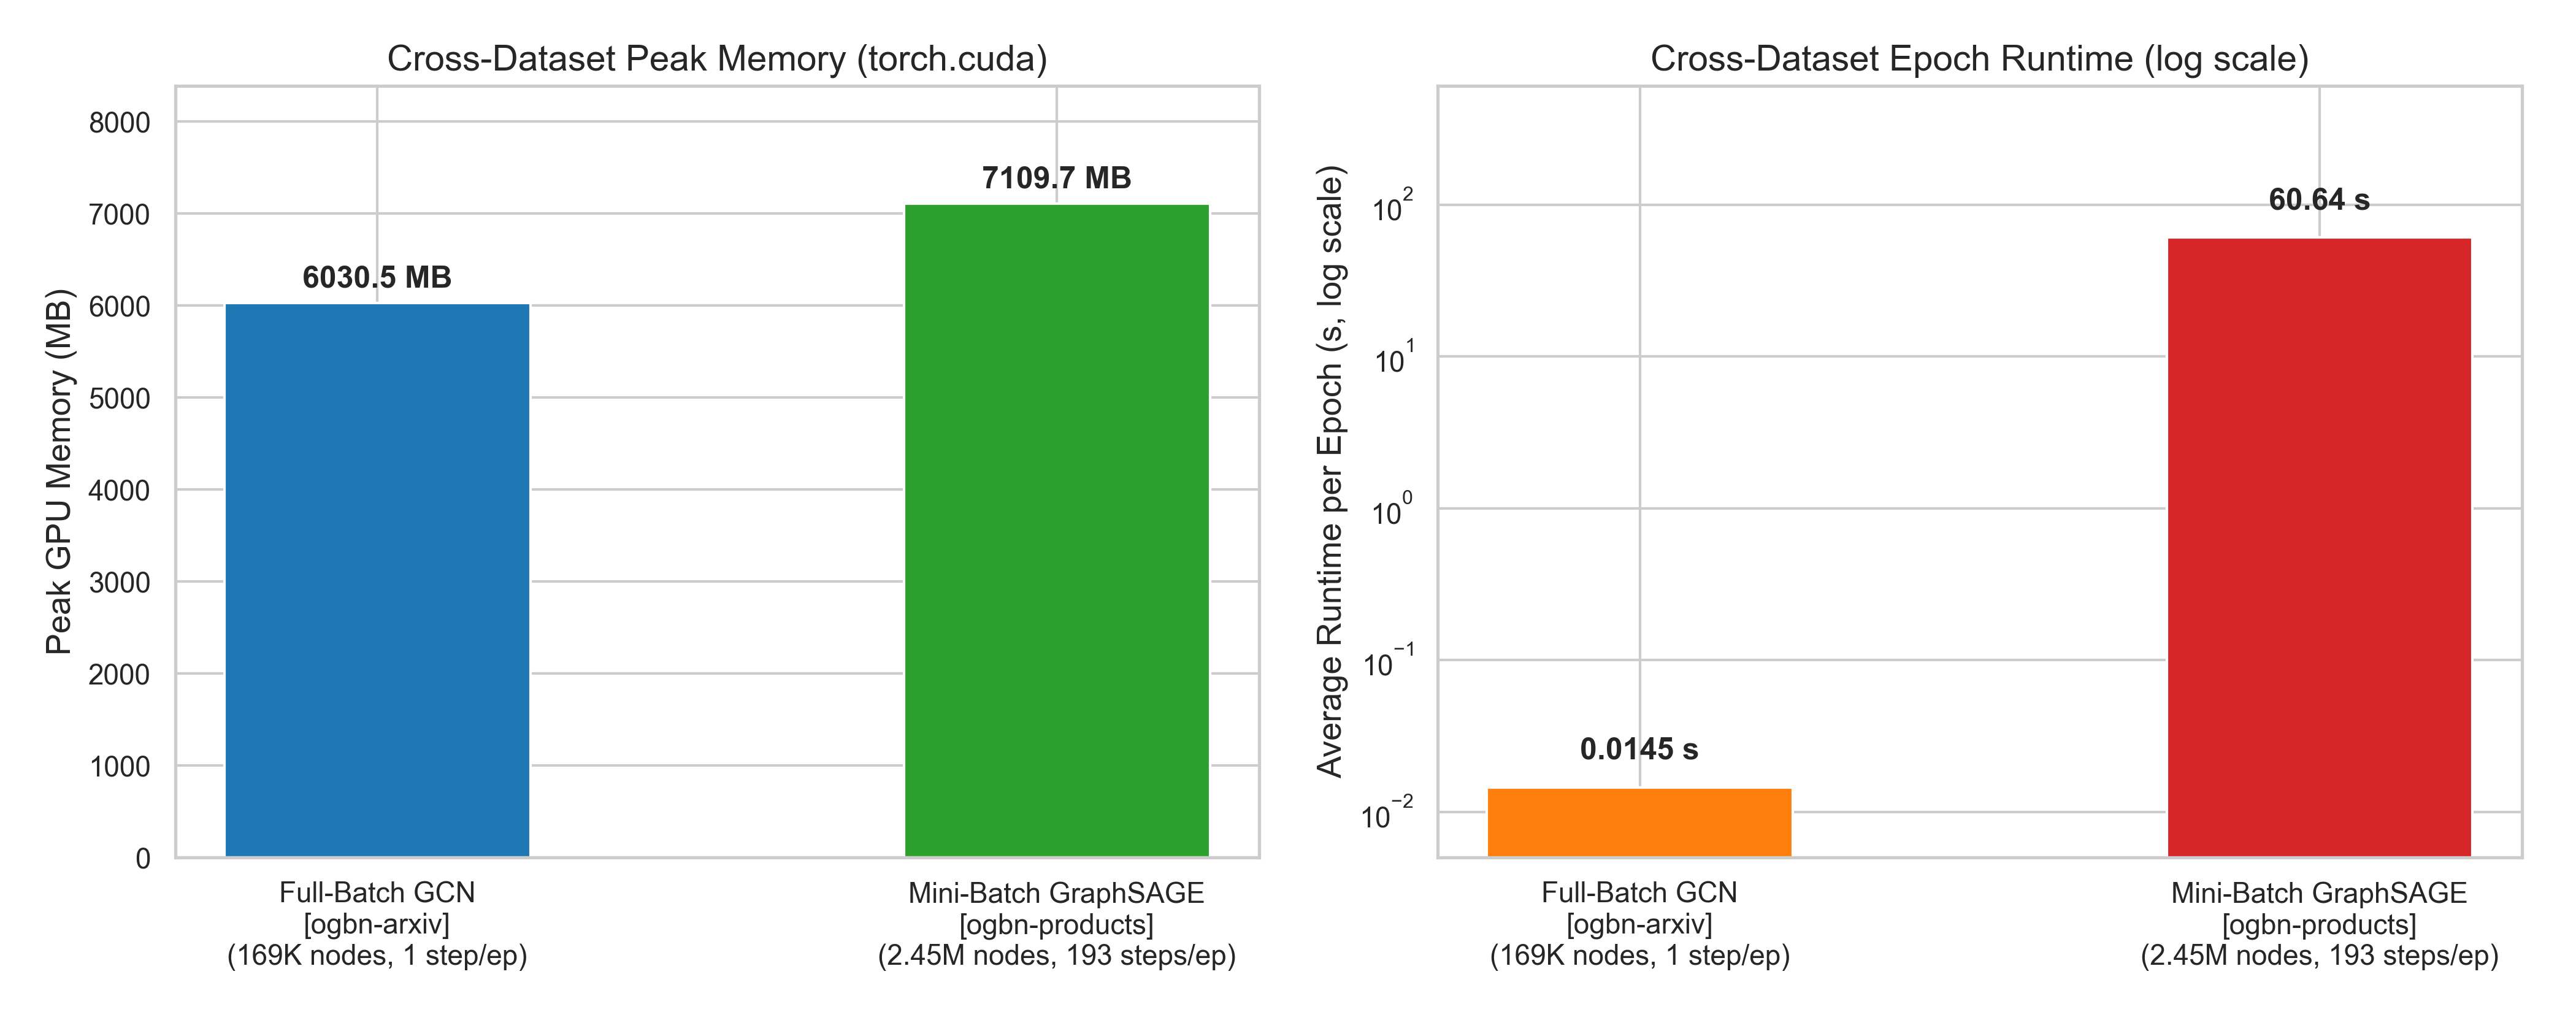
\includegraphics[width=0.98\columnwidth]{comparative_profiling.png}
    \caption{Peak GPU memory and epoch runtime for GCN (\texttt{ogbn-arxiv})
             and GraphSAGE (\texttt{ogbn-products}) across configurations.}
    \label{fig:profiling}
\end{figure}

\subsection{Memory Scaling \& OOM Extrapolation}
From the depth ablation (Table~\ref{tab:gcn_ablation}), GCN activation memory
grows by ${\approx}585$ MiB per layer on \texttt{ogbn-arxiv} ($|V|{=}169$K).
Scaling to \texttt{ogbn-products} ($|V|{=}2.45$M, a $14.5{\times}$ increase):
\begin{equation}
  \Delta M_{\text{layer}} \approx 585\text{ MiB} \times 14.5 \approx 8.3\text{ GiB/layer}
\end{equation}
A 3-layer model requires $\approx 24.9$ GiB for activation caching alone (a
\emph{lower bound}: this excludes the ${\approx}4.2$ GiB baseline offset visible
at $L{=}0$ extrapolation and unattributed full-graph evaluation buffers;
\texttt{max\_memory\_allocated} counts only live tensors, not cached-but-free
reserved blocks).  Adding the symmetrized \texttt{edge\_index} for 61.8M
undirected edges ($123.7$M directed pairs $\times 2 \times 8$ bytes
$\approx 1.84$ GiB) and intermediate aggregation buffers pushes the true
requirement well beyond 30 GiB.

Empirically, running full-batch GCN on \texttt{ogbn-products} on a Tesla T4
(16 GB, 14.75 GiB usable) terminates immediately with:

\begin{verbatim}
torch.cuda.OutOfMemoryError:
  Tried to allocate 9.16 GiB
  (5.47 GiB already allocated;
   102 MiB free; 9.24 GiB reserved)
\end{verbatim}

The remaining $\approx5.4$ GiB of total VRAM (14.75 GiB) was unavailable to
PyTorch at launch (likely a stale process or prior notebook state holding GPU
memory; the exact cause is unconfirmed without a fresh \texttt{nvidia-smi}
reading). In contrast, mini-batch GraphSAGE trains stably on the same GPU
($6.9$ GiB peak, or only $3.6$ GiB with $S=[5,5,5]$).

\subsection{Why Stochastic Sampling Prevents Neighborhood Explosion}

\paragraph{Full-Batch Memory Bottleneck:}
Full-batch GCN computes $H^{(l+1)} = \sigma(\tilde{A}_{\text{norm}} H^{(l)} W^{(l)})$
globally. Backpropagation requires retaining all $L$ activation tensors
$\{H^{(0)},\ldots,H^{(L)}\}$, imposing $\mathcal{O}(L \cdot |V| \cdot d)$ memory
that \emph{grows linearly with graph size}.  Moreover, naive node-level
mini-batching without sampling fails: in a power-law graph with average degree
$\bar{d}\approx 50.5$ (\texttt{ogbn-products}), an $L=3$ unconstrained expansion
yields $(50.5)^3 \approx 1.28{\times}10^5$ neighborhood walks per seed node, such
that mini-batch neighborhoods can cover a large fraction of the graph.

\paragraph{Stochastic Neighborhood Sampling:}
GraphSAGE caps the sample budget at each hop $l$ to a fixed $S_l$. For a
mini-batch of $B$ seed nodes, the frontier at hop $L$ is bounded by
\begin{equation}
  |\mathcal{V}_L| \le B \cdot \prod_{l=1}^L S_l
\end{equation}
and the total sampled nodes are bounded by $B\bigl(1+\sum_{l=1}^L \prod_{i=1}^l
S_i\bigr)$.  Per-step backpropagation memory is thus
$\mathcal{O}\!\bigl(B \cdot d \cdot \prod_{l=1}^L S_l\bigr)$, which is
\textbf{independent of $|V|$}.  Static node features occupy $\mathcal{O}(|V|{\cdot}d)$
memory ($\approx 934$ MiB here); in out-of-core pipelines these can reside in host
memory while only per-step activation tensors are on-device. Gradient computation
is thus bounded by the sampled subgraph, enabling scalable training on graphs of
arbitrary size.

% =============================================================================
\section{Reproducibility \& Environment}
% =============================================================================
All experiments ran on an NVIDIA Tesla T4 (16 GB, 14.75 GiB usable; 2 vCPUs),
Python 3.11, PyTorch 2.1.0, PyG 2.4.0, OGB 1.3.6. Memory quantities labelled
``MB'' in tables use binary prefixes (MiB) as returned by
\texttt{torch.cuda.max\_memory\_allocated()}. Seed 42 was used for all single-run
baselines and ablations; seeds 42--46 for the GCN multi-seed evaluation.
GCN per-epoch time ($14.5$ ms) averages the forward pass, backward pass, and
optimizer step in FP32 with \texttt{torch.cuda.synchronize()}, excluding
evaluation overhead. GraphSAGE times include sampling and training but exclude
periodic evaluation passes. Full code, scripts, and the OOM log are at
\url{https://github.com/vaishvi-code/CSC591-038-_hw2}.

% =============================================================================
\section{Conclusion}
% =============================================================================
We successfully reproduced GCN on \texttt{ogbn-arxiv} ($71.15\%{\pm}0.26\%$
test, vs.\ official $71.74\%{\pm}0.29\%$) and GraphSAGE on \texttt{ogbn-products}
($78.61\%$ test, vs.\ official $78.70\%{\pm}0.36\%$). Hyperparameter analysis
shows that GCN validation accuracy peaks at $L=4$, though the gain over $L=3$
is within run-to-run noise and test accuracy peaks at $L=3$; performance drops
genuinely beyond $L=4$, hypothesized as oversmoothing or gradient attenuation.
Learning rates of $0.005$--$0.010$ are nearly equivalent ($0.01$ pp test gap).
For GraphSAGE, front-loading neighbor budgets ($S=[15,5,5]$) achieves
comparable validation accuracy to the baseline at $1.3{\times}$ lower memory
and $1.6{\times}$ faster runtime, though test accuracy is $0.60$ pp lower
($77.29\%$ vs.\ $77.89\%$, roughly $1.7{\times}$ the OGB std). Aggressive
reduction to $S=[5,5,5]$ provides a $3.5{\times}$ speedup at $\approx 2$ pp
test cost. Profiling confirms that stochastic sampling decouples per-step activation
memory from graph size; full-batch GCN is projected to need ${\approx}25$ GiB
for \texttt{ogbn-products} and ran out of memory on our T4 (14.75 GiB usable).

\end{document}
